\section{Messung}
\label{sec:messung}
Im Folgenden Abschnitt wird zunächst eine Energiekalibration der Apparatur durchgeführt. Anschließend werden mit der Aufnahme eines Cäsium-Strahlers verschiedene Detektoreigenschaften bestimmt.
Daraufhin wird die Aktivität einer ???-Quelle gemessen und schließlich einige Holzkohlebriketts auf ihre radioaktiven Bestandteile untersucht.

\subsection{Eichung und Effizienz des Ge-Detektors}
\label{subse:eichung}
Wie in Abschnitt \ref{sub:bestimmung_der_energie_und_der_aktivität_einer_gamma_quelle} erwähnt, liegen nach der Messung lediglich Informationen über einen Energiekanal vor, in dem ein Ereignis detektiert wurde.
Um das entsprechende Spektrum in der Dimension \si{keV} der Energie zu erhalten, wird den Kanälen $C$ mit einer lineare Kalibrationsfunktion $E(C)$ eine jeweilige Energie $E$ zugeordnet.
Mit der Steigung $m$ und einem Offset $b$ wird hierfür verwendet:%
%
\begin{align}
    \label{eqn:kalibration}
    E(C) = mC + b\,.
\end{align}

Zunächst wird das Spektrum eines $^{52}$Eu-Strahlers aufgenommen (Abb. \ref{fig:eu_uncalibrated}).
Um den Einfluss von Untergrundereignisse zu verringern, wird zudem eine Leermessung durchgeführt und die Einträge dieser Messung der einzelnen Kanäle von dem Spektrum des $^{52}$Eu-Strahlers abgezogen (Abb. \ref{fig:leermessung}).
\begin{figure}[htb]
    \centering
    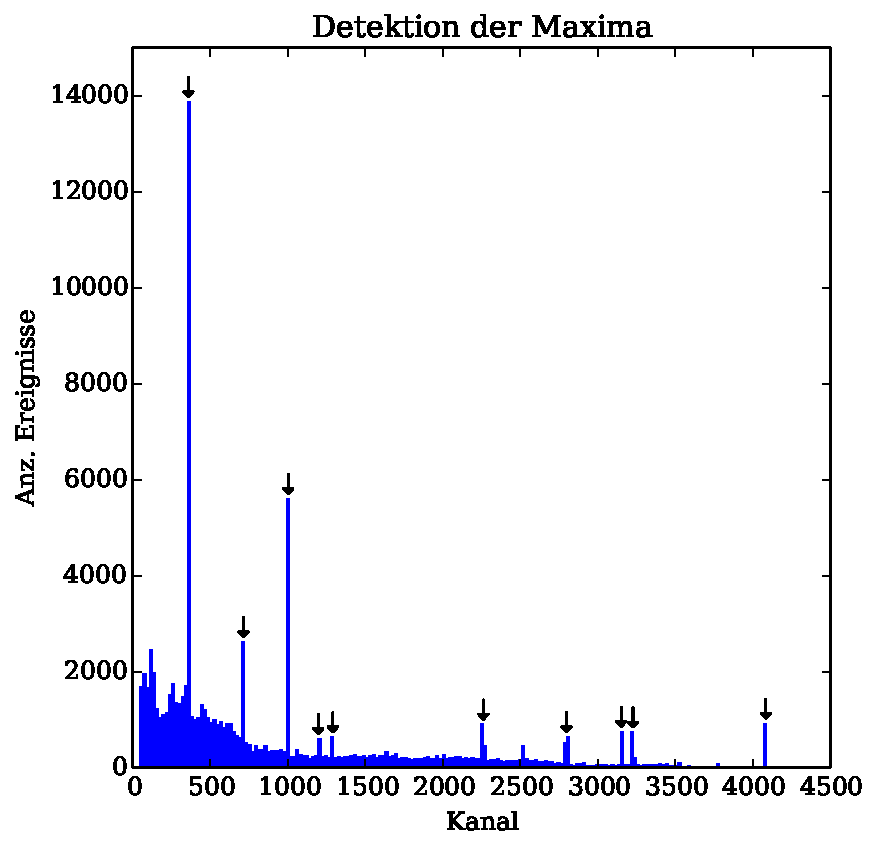
\includegraphics[width=0.8\textwidth]{img/02_maxima.pdf}
    \caption{
        Energiespektrum des $^{52}$Eu-Strahlers. Die zur Energiekalibration genutzten Maxima im Spektrum sind mit einem Pfeil markiert.
    }
    \label{fig:eu_uncalibrated}
\end{figure}
Die unterschiedliche Messdauer wird mit einem Faktor $t_\text{leer} / t_\text{Eu}$ der Messdauer $t_\text{Eu}$ des $^{52}$Eu-Strahlers und $t_\text{leer}$ der Leermessung berücksichtigt.
Für die Kalibration werden die in Tabelle \ref{tab:maxima} aufgeführten Maxima gewählt und den jeweiligen Kanäle mit Hilfe von \eqref{eqn:kalibration} eine Energie zugeordnet. Der Fit der Kalibratinosfunktion ist in Abbildung \ref{fig:calibration} dargestellt.
Es ergeben sich die Koeffizienten
%
\begin{align*}
     m = \SI{345.22+-0.04}{keV/C} \qquad b = \SI{-1.82+-0.09}{keV} \,.
\end{align*}

Nach der Kalibration des Gerätes, kann die Effizienz $Q$ wie in Abschnitt \ref{sub:bestimmung_der_energie_und_der_aktivität_einer_gamma_quelle} beschrieben bestimmt werden. Mit Gleichung \eqref{eqn:raumwinkel} ergibt sich ein Raumwinkelanteil des Detektors von
\begin{align*}
    \frac{\Omega}{4\pi} = \num{0.443+-0.006}
\end{align*}

\begin{table}[htb]
    \centering
    \caption{
        Die für die Kalibration des Ge-Detektors verwendeten Maxima des $^{52}$Eu-Spektrums.
    }
    \label{tab:maxima}
    \begin{tabular}{%
        S[table-format=3.2]%
        S[table-format=3.2]%
        S[table-format=3.2]%
    }
        \toprule
        {Energie [\si{keV}]} &
        {Emissionsw. [\si{\percent}]} &
        {Kanal} \\
        \midrule
        121.78 & 28.6 &  358 \\
        244.7  &  7.6 & 1003 \\
        344.3  & 26.5 &  714 \\
        411.12 & 02.2 & 2262 \\
        443.96 & 03.1 & 2798 \\
        778.9  & 12.9 & 4084 \\
        964.08 & 14.6 & 3227 \\
        1085.9 & 10.2 & 1291 \\
        1112.1 & 13.6 & 3150 \\
        1408.0 & 21.0 & 1196 \\
        \bottomrule
    \end{tabular}
\end{table}
